\chapter{Metodología}
\label{ch:metodologia}

En el presente capítulo se presentará la metodología utilizada para la creación de un modelo propuesto para la predicción de demanda y maximización de ingresos en hoteles. La metodología guiará la estructura de este trabajo con el fin de hacer de él una contribución científica. La presente investigación se puede dividir en dos partes. La primera, consistió en el desarrollo un modelo capaz de predecir la demanda y ofrecer recomendaciones de precios para maximizar el ingreso diario de una propiedad. La segunda parte consistió en probar dicho modelo y discutir los resultados obtenidos con la finalidad de abrir nuevas líneas de investigación.

\section*{Diseño del modelo}

Para construír un modelo de predicción de demanda y maximización de ingresos para los hoteles que fueron sujetos al estudio, se siguió la metodología \emph{CRISP DM} la cual se compone de una serie de pasos descritos a continuación:

\begin{figure}[H]
  \centering
      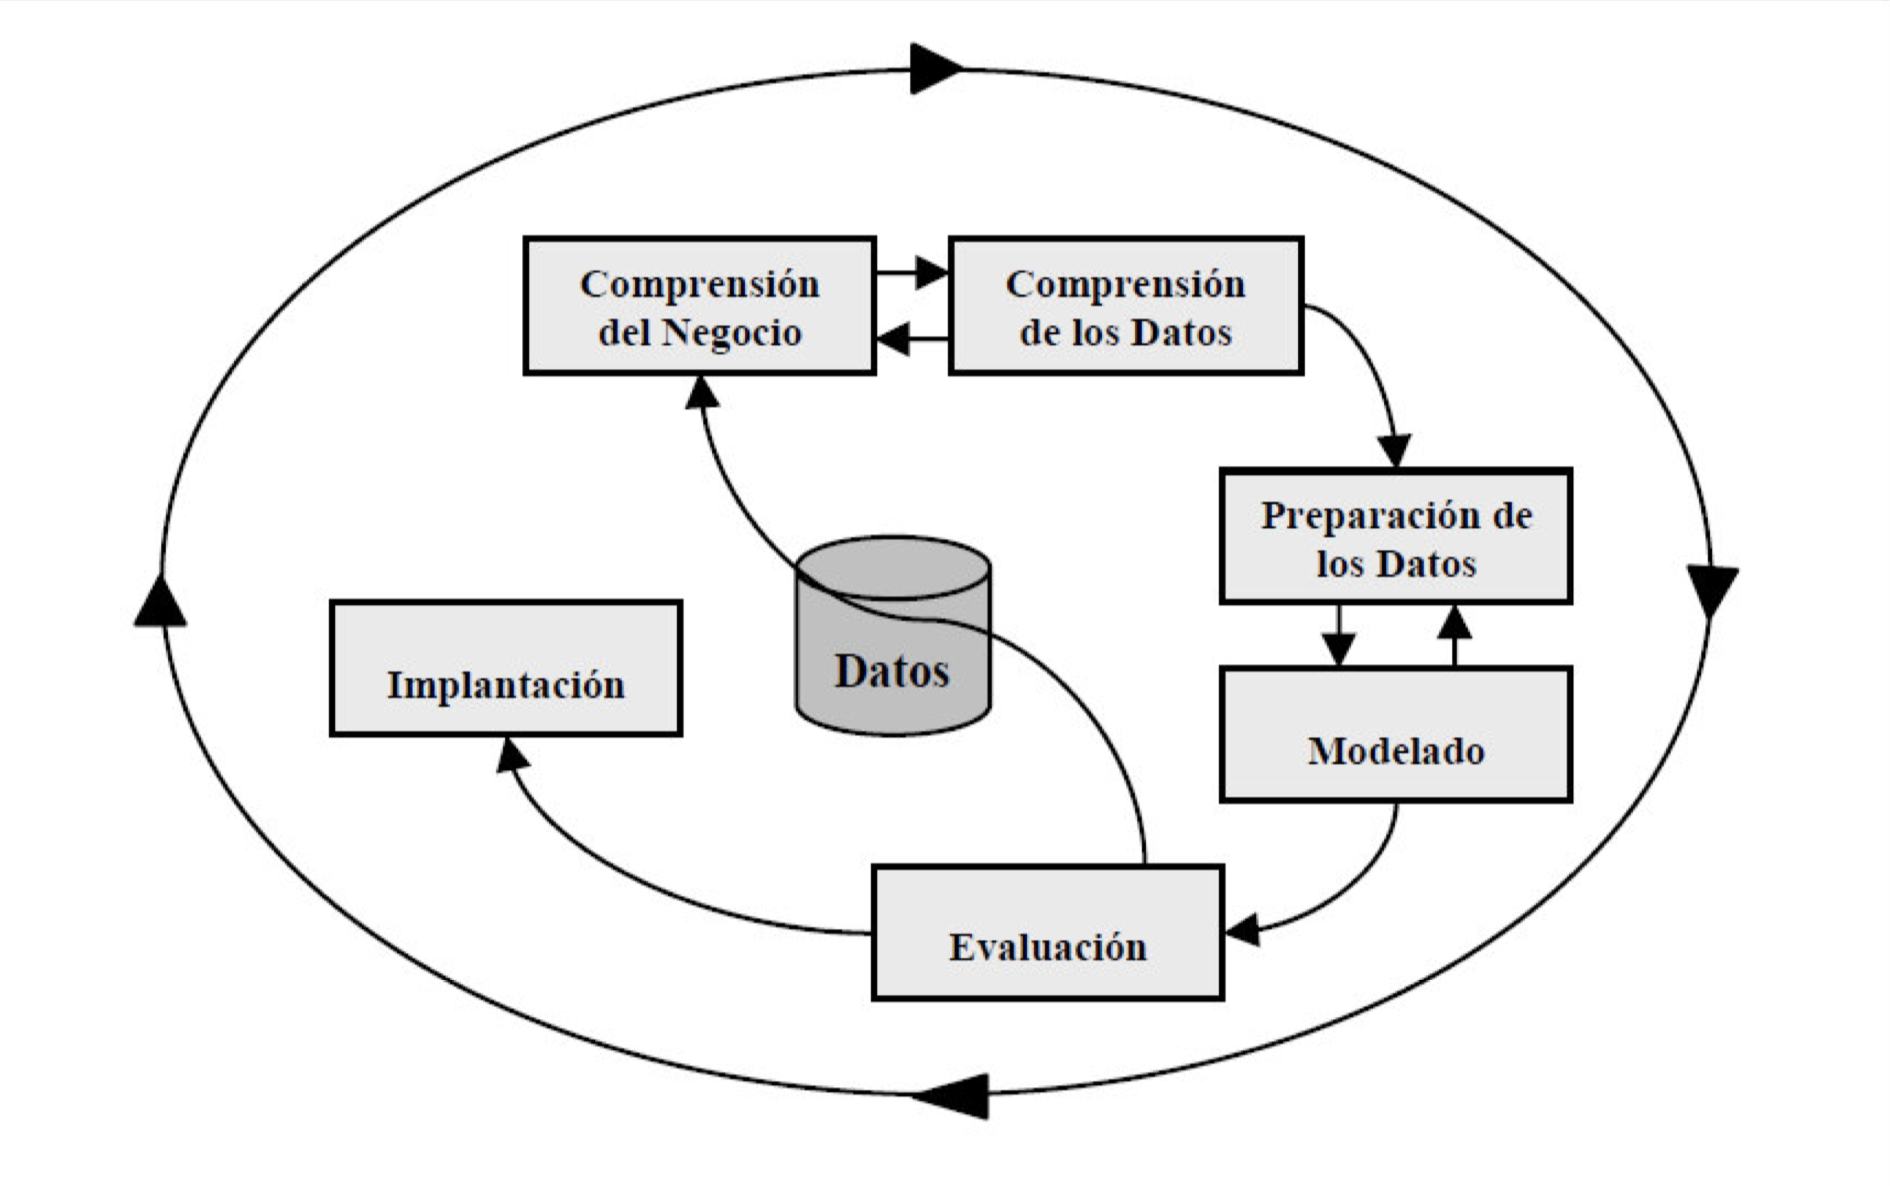
\includegraphics[width=\maxwidth,height=8cm]{figures/crisp.png} 
  \caption{Modelo de proceso CRISP–DM [CRISP-DM, 2000]}
\end{figure}

\subsubsection*{Comprensión del negocio}

El primer paso durante la construcción del modelo fue el entendimiento del negocio ya que para poder interpretar los datos es necesario comprender el negocio que está implícito en ellos. Durante esta etapa se trabajó con el equipo de gestión comercial de las propiedades para entender qué datos son analizados durante el proceso de toma de decisiones; de dónde son obtenidos y qué variables son de mayor interés para el negocio.

\subsubsection*{Identificación de las fuentes de datos}

Una vez comprendido el negocio y detectadas las variables de interés durante el proceso de la toma de decisiones, se identificaron las fuentes de datos, las cuales son nutridas por dos principales sistemas dentro de las propiedades: la central de reservaciones y el sistema de gestión de la propiedad. El primero sirve para dar servicio a todos los huéspedes que buscan una habitación mediante los canales de reservación disponibles (sitio web, call center, aplicaciones móviles, correos electrónicos, etc) y el segundo gestiona la propiedad y dá servicio al huésped desde que llega hasta que se retira de la propiedad. Estos sistemas contienen toda la información del proceso desde que se encuentra en estatus de reservación hasta que llega a un estatus de \emph{check out}.

\subsubsection*{Comprensión de los datos}

Luego de haber identificado las principales fuentes de datos, se diseñaron los procesos de extracción de información necesarios para obtener los datos que serían utilizados para la construcción del modelo. Para entender los datos, se ejecutó un análisis exploratorio, en dónde se observó el comportamiento de las variables de interés, su distribución probabilística, temporalidades presentes, nível de limpieza y datos atípicos que pudieran generar problemas al momento de la implementación del modelo final.

\subsubsection*{Prepración de los datos - modelado}

Para la construcción del modelo se tuvieron varias iteraciones en el desarrollo. La primera, consistió en el diseño de los procesos \emph{ETL} para la construcción de los \emph{sets de datos} que alimentan a los tres modelos de pronóstico de demanda propuestos. La segunda iteración se enfocó en la construcción de los tres modelos de pronóstico de demanda, durante esta etapa se analizaron distintos enfoques como: regresiones lineales generalizadas, modelos de series de tiempo (ARIMA) y finalmente la regresión de Ridge. Durante la tercera iteración se construyó el modelo de optimización de ingresos. Este modelo toma como datos de entrada los resultados obtenidos por el modelo de predicción de demanda y como resultado arroja recomendaciones de precios para la tarifa publica. La última iteración consisitó en la ejecución de el modelo integral para poder medir el desempeño y poder obtener los resultados finales.

\subsection*{Evaluación}

Durante esta etapa se ejecutó el modelo para pronósticar la demanda y maximizar los ingresos para un mes posterior a la fecha de ejecución, los resultados fueron comparados con el desempeño real de la propiedad para obtener el \emph{MAPE} del modelo construído. En el capítulo de \emph{Resultados} del presente trabajo se presentarán los detalles de las pruebas ejecutadas y los resultados obtenidos.
